\documentclass[border=10pt]{standalone}

\usepackage{tikz}
\usepackage{tikzsymbols}
\usetikzlibrary{calc,patterns,shapes.geometric}

\def\centerarc[#1](#2)(#3:#4:#5){\draw[#1] ($(#2)+({#5*cos(#3)},{#5*sin(#3)})$) arc (#3:#4:#5);}

\begin{document}
	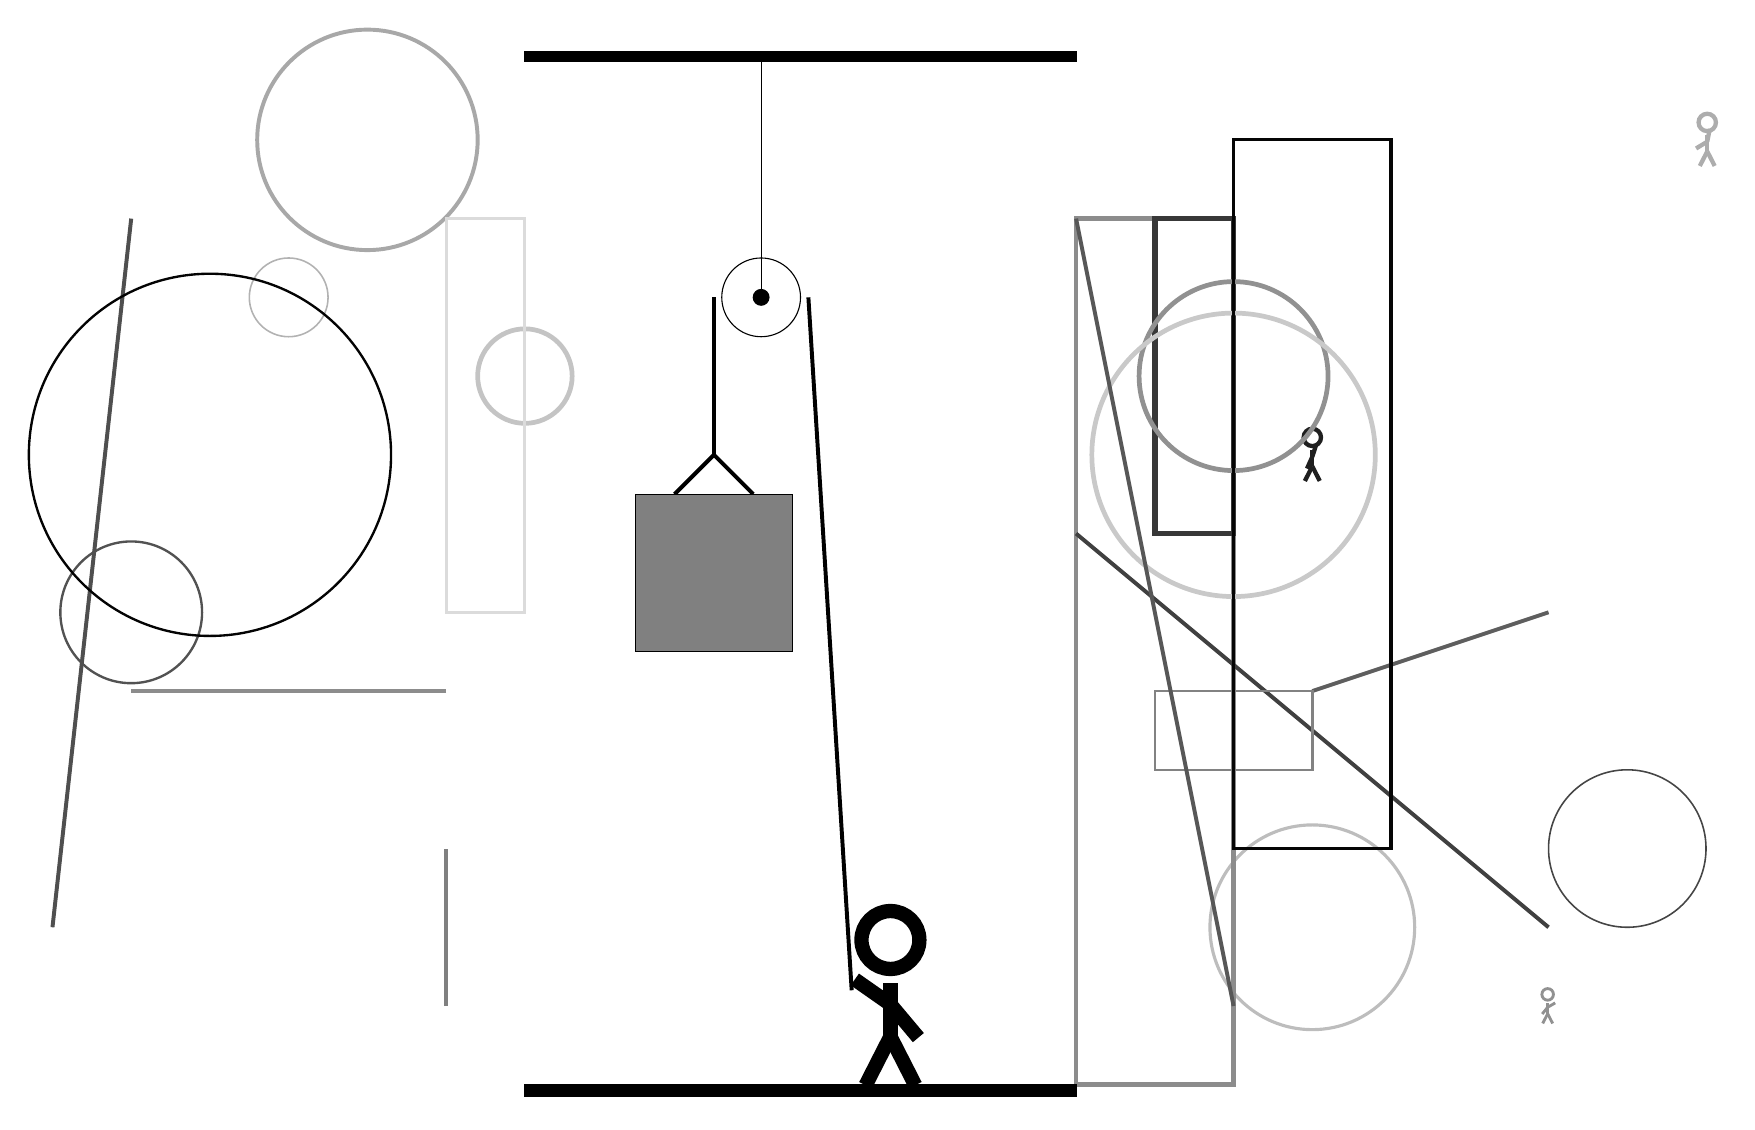
\begin{tikzpicture}
		%%%%% START %%%%%
		
		\draw[fill=black] (-2, 10) rectangle (5, 10.125);
		
		\draw (1, 7) circle (0.5);
		\draw[fill=black] (1, 7) circle (0.1);
		\draw (1, 10) -- (1, 7);
		
		\draw[line width=0.5mm] (-0.1, 4.5) -- (0.4, 5.0) -- (0.9, 4.5);
		\draw[fill=black!50] (-0.6, 4.5) rectangle (1.4, 2.5);
		
		\draw[line width=0.5mm] (0.4, 7) -- (0.4, 5.0);
		\centerarc[line width=0.5mm](1, 7)(0:180:0.6);
		\draw[line width=0.5mm](1.6, 7) -- (2.15, -1.8);
		
		\node at (2.6, -1.9) {\Strichmaxerl[10][-35][-50]};
		
		\draw[line width=0.5mm, color=black!63](8, 2) -- (11, 3);
		
		\draw [line width=0.4mm, color=black!26](8, -1) circle (1.3);
		\draw [line width=0.2mm, color=black!30](-5, 7) circle (0.5);
		\draw [line width=0.2mm, color=black!73](12, 0) circle (1.0);
		\draw [line width=0.6mm, color=black!23](-2, 6) circle (0.6);
		
		\node[line width=0.6mm, color=black!43] at (11, -2) {\Strichmaxerl[2][51][30]};
		
		\draw[line width=0.6mm, color=black!45] (7, -3) rectangle (5, 8);
		\draw [line width=0.5mm, color=black!34](-4, 9) circle (1.4);
		\draw[line width=0.5mm, color=black!75](5, 4) -- (11, -1);
		
		\draw[line width=0.4mm, color=black!14] (-3, 8) rectangle (-2, 3);
		
		\draw[line width=0.5mm, color=black!50](-3, -2) -- (-3, 0);
		
		\draw[line width=0.3mm, color=black!49] (6, 2) rectangle (8, 1);
		\node[line width=0.7mm, color=black!32] at (13, 9) {\Strichmaxerl[3][31][79]};
		
		\draw[line width=0.5mm, color=black!45](-3, 2) -- (-7, 2);
		\draw [line width=0.3mm, color=black!68](-7, 3) circle (0.9);
		\node[line width=0.7mm, color=black!88] at (8, 5) {\Strichmaxerl[3][66][72]};
		
		\draw[line width=0.7mm, color=black!78] (6, 4) rectangle (7, 8);
		
		\draw [line width=0.6mm, color=black!43](7, 6) circle (1.2);
		\draw[line width=0.5mm, color=black!69](-7, 8) -- (-8, -1);
		\draw [line width=0.3mm, color=black!99](-6, 5) circle (2.3);
		\draw [line width=0.6mm, color=black!21](7, 5) circle (1.8);
		
		\draw[line width=0.2mm, color=black!15] (5, 6) rectangle (5, 6);
		
		\draw[line width=0.5mm, color=black!66](5, 8) -- (7, -2);
		\draw[line width=0.4mm, color=black!98] (7, 0) rectangle (9, 9);
		
		\draw[fill=black] (-2, -3) rectangle (5, -3.15);
		
		%%%%% END %%%%%
	\end{tikzpicture}
\end{document}